% ========================================================================
% 
% DOCTORAL THESIS
% Possibilities of use of artificial neural networks in work with spatial data
% 
% Ondřej Pešek
% 
% ========================================================================

\documentclass[
  12pt,         			% velikost základního písma je 12 bodů
  a4paper,      			% formát papíru je A4
  oneside,       			% Oboustranný tisk
  pdftex,				    % překlad bude proveden programem 'pdftex' do PDF
  english,
  %draft
]{report}       			% dokument třídy 'zpráva'


\newcommand{\Fbox}[1]{\fbox{\strut#1}}

\usepackage[english, czech]{babel}	% použití češtiny, angličtiny
\usepackage[utf8]{inputenc}			% kódování zdrojových souborů je UTF8

\usepackage[square,sort,comma,numbers]{natbib}

\usepackage{caption}
\usepackage{subcaption}
\usepackage{listings}

\usepackage[dvipsnames]{xcolor}
\definecolor{light-gray}{gray}{0.95}

\captionsetup{font=small}
\usepackage{enumitem}
\setlist{leftmargin=*} % bez odsazení

\makeatletter
\setlength{\@fptop}{0pt}
\setlength{\@fpbot}{0pt plus 1fil}
\makeatletter

\usepackage[dvips]{graphicx}   
\usepackage{color}
\usepackage{transparent}
\usepackage{wrapfig}
\usepackage{float} 

\usepackage{cmap}           
\usepackage[T1]{fontenc}    

\usepackage{textcomp}
\usepackage[compact]{titlesec}
\usepackage{amsmath}
\addtolength{\jot}{1em} 

\let\counterwithout\relax
\let\counterwithin\relax
\usepackage{chngcntr}
\counterwithout{footnote}{chapter}

\usepackage{acronym}

\usepackage[
    unicode,                
    breaklinks=true,        
    hypertexnames=false,
    colorlinks=true, % true for print version
    citecolor=black,
    filecolor=black,
    linkcolor=black,
    urlcolor=black
]{hyperref}         

\usepackage{url}
\usepackage{fancyhdr}
% \usepackage{algorithmic}
\usepackage{algorithm}
\usepackage{algcompatible}
\renewcommand{\ALG@name}{Pseudocode}% update algorithm name
\def\ALG@name{Pseudocode}

\usepackage[
  cvutstyle,          
  phd,
  english
]{thesiscvut}


\newif\ifweb
\ifx\ifHtml\undefined % mimo HTML.
    \webfalse
\else % v HTML.
    \webtrue
\fi 

\renewcommand{\figurename}{Obrázek}
\def\figurename{Obrázek}

\lstdefinestyle{python}{
   language=python,
   basicstyle={\footnotesize\ttfamily},
   keywordstyle=\color{blue}\ttfamily,
   stringstyle=\color{green}\ttfamily,
   commentstyle=\color{brown}\ttfamily,
   showstringspaces=false,
   morekeywords={True, False, sqrt}
}

%\renewcommand\lstlistingname{Pseudocode}
%\renewcommand*{\lstlistlistingname}{Content of pseudocodes}

\usepackage{dirtree}

\lstset{
	extendedchars=true,
	literate={á}{{\'a}}1}

\makeatletter
\newcommand\footnoteref[1]{\protected@xdef\@thefnmark{\ref{#1}}\@footnotemark}
\makeatother

\usepackage{tikz}
\usetikzlibrary{arrows.meta, shapes}
\tikzset{%
  >={Latex[width=1mm,length=1mm]},
  % Specifications for style of nodes:
            base/.style = {rectangle, rounded corners, draw=black,
                           minimum width=4cm, minimum height=1cm,
                           text centered, font=\sffamily},
  activityStarts/.style = {base, fill=blue!30},
       startstop/.style = {base, fill=red!30},
    activityRuns/.style = {base, fill=green!30},
    test/.style = {base, diamond, aspect=2, text width=8em, fill=yellow!30},
         process/.style = {base, minimum width=2.5cm, fill=orange!15,
                           font=\ttfamily},
}

\usepackage[justification=centering]{caption}

\newcommand\textstyleEmphasis[1]{\textit{#1}}
\newcommand\liststyleLi{%
\renewcommand\labelitemi{{\textbullet}}
\renewcommand\labelitemii{{\textbullet}}
\renewcommand\labelitemiii{{\textbullet}}
\renewcommand\labelitemiv{{\textbullet}}
}
\newcommand\liststyleLii{%
\renewcommand\labelitemi{{\textbullet}}
\renewcommand\labelitemii{{\textbullet}}
\renewcommand\labelitemiii{{\textbullet}}
\renewcommand\labelitemiv{{\textbullet}}
}

\newcommand\tab[1][1cm]{\hspace*{#1}}

% ========================================================================
% Definice informací o dokumentu
% ========================================================================

% název práce
\nazev{Possibilities of use of artificial neural networks in work with spatial data}
{Možnosti využití umělých neuronových sítí v práci s~prostorovými daty}

% jméno a příjmení autora
\autor{Ing. Ondřej}{Pešek}

% jméno a příjmení vedoucího práce včetně titulů
\garant{Prof. Aleš Čepek,~CSc.; Ing. Martin Landa,~PhD.}

% označení oboru studia
\oborstudia{Geomatics}{}

% označení ústavu
\ustav{Department of Geomatics}{}

% rok obhajoby
\rok{2020}

% měsíc obhajoby
\mesic{}

% místo obhajoby
\misto{Prague}

% abstrakt
\abstrakt 
{In recent years, the speed of technological progress in certain science fields is getting faster and faster. It is making it hard for other scientific areas to keep up with this tempo. One of the~exemplary relationships is the link between artificial neural network structures and the province of geomatics or remote sensing. New architectures of artificial neural network models are being published with an expeditious tempo and the common approach of the~remote sensing researchers is to use the most recent structures, without the~basic understanding of the background or relative performance. The goal of this thesis is to perform systematic research on the possibilities of use of chosen artificial neural network architectures on various selected use cases from the field of remote sensing.}
{Technologický vývoj v některých vědních odvětvích nabírá v posledních několika letech stále na rychlosti. A pro ostatní vědní obory je těžké držet s okolím tempo. Jedním takovým vztahem jsou struktury umělých neuronových sítí a obor geomatiky, případně dálkového průzkumu Země. Nové architektury modelů umělých neuronových sítí se objevují nebývalým kvapem, a běžný přístup výzkumníků dálkového průzkumu Země bývá ten, že si pro zpracovávání dat vybírají bez větší znalosti pozadí či porovnání nejnovější modely. Cílem této doktorské práce je systematicky prozkoumat a porovnat možnosti využití určených architektur umělých neuronových sítí na vybraných aplikačních tématech z prostředí dálkového průzkumu Země.}


% klíčová slova
\klicovaslova
{artificial neural networks, convolutional neural networks}
{umělé neuronové sítě, konvoluční neuronové sítě}

% ========================================================================
% Nastavení polí ve vlastnostech dokumentu PDF
% ========================================================================
\nastavenipdf

% začátek dokumentu
\begin{document}

\catcode`\-=12  % pro vypnutí aktivního znaku '-' používaného např. v \cline 

% aktivace záhlaví
\zahlavi

% předefinování vzhledu záhlaví
\renewcommand{\chaptermark}[1]{%
	\markboth{\MakeUppercase
	{%
	\thechapter.%
	\ #1}}{}}

% vysázení přebalu práce
%\vytvorobalku

% vysázení titulní stránky práce
\vytvortitulku

% Vysázení listu zadani
\stranka{}%
	%{\includegraphics[scale=0.7]{./pictures/zadanidp.pdf}}%\sffamily\Huge\centering\ }%ZDE VLOŽIT LIST ZADÁNÍ}%
	%{\sffamily\centering Z~důvodu správného číslování stránek}

% vysázení stránky s abstraktem
\vytvorabstrakt

% vysázení prohlaseni o samostatnosti
%\vytvorprohlaseni

% vysázení poděkování
%\stranka{%nahore
%       }{%uprostred
%       }{%dole
%       \sffamily
%	\begin{flushleft}
%		\large
%		\MakeUppercase{Acknowledgement}
%	\end{flushleft}
%	\vspace{1em}
%		%\noindent
%	\par\hspace{2ex}
%	{I would like to thank my parents for their support during my studies.
%	Then I would like to thank Martin Landa, not only for supervising my thesis
%	but also for the initial impulse in the direction to artificial neural
%	networks and open source GIS generally. My thanks also belong to Margherita Di
%	Leo for long initial discussions about the usage of neural networks in the
%	field of GIS, to Moritz Lennert for testing and comments during the code
%	sprint in Bonn, and to Luca Delucchi and Fondazione Edmund Mach for
%	the~willingness to exploit their time and resources to test modules.}
%}

% vysázení obsahu
% \setcounter{tocdepth}{1}
\obsah

% vysázení seznamu obrázků
%\seznamobrazku

% vysázení seznamu tabulek
% \seznamtabulek

% vysázení seznamu ukázek kódu
%\cleardoublepage
%\thispagestyle{empty}
% \lstlistoflistings
%\newpage

% jednotlivé kapitoly
\chapter{Introduction}
\label{intro}

The future is arriving faster than we think. The technological progress is accelerating. Human knowledge is growing faster than ever before. If citing slightly lurid sources, according to Fuller's knowledge doubling curve \cite{knowledge-doubling-curve}, it took about 1500 years starting at the year 1 for the society amount of knowledge to double itself, then the doubling needed just about 100 years around the year 1900, and only 10 years around the year 1960; according to \cite{growth-forecast}, the knowledge doubled every 1.5 years around the year 2011. Besides many other aspects of such an information growth, it opens gates for technologies previously only dreamed up. Technologies like the artificial intelligence (\zk{AI}).

Artificial neural networks (\zk{ANN}s) became a term that is shaking the entire field of computer science. In the field of computer vision, it is especially their special type called convolutional neural networks (\zk{CNN}s) that is outperforming classical approaches to object detection and segmentation \cite{cnn-off-the=shelf}. Therefore, it should not be a surprise that \zk{ANN}s are widely used also in the field of remote sensing already since 2014 \cite{review-dl-rs-2017}, and their use outside and inside the field is just growing, as can be seen in figures \ref{fig-dl} and \ref{fig-rs-dl}.

\begin{figure}[h]
   \centering
	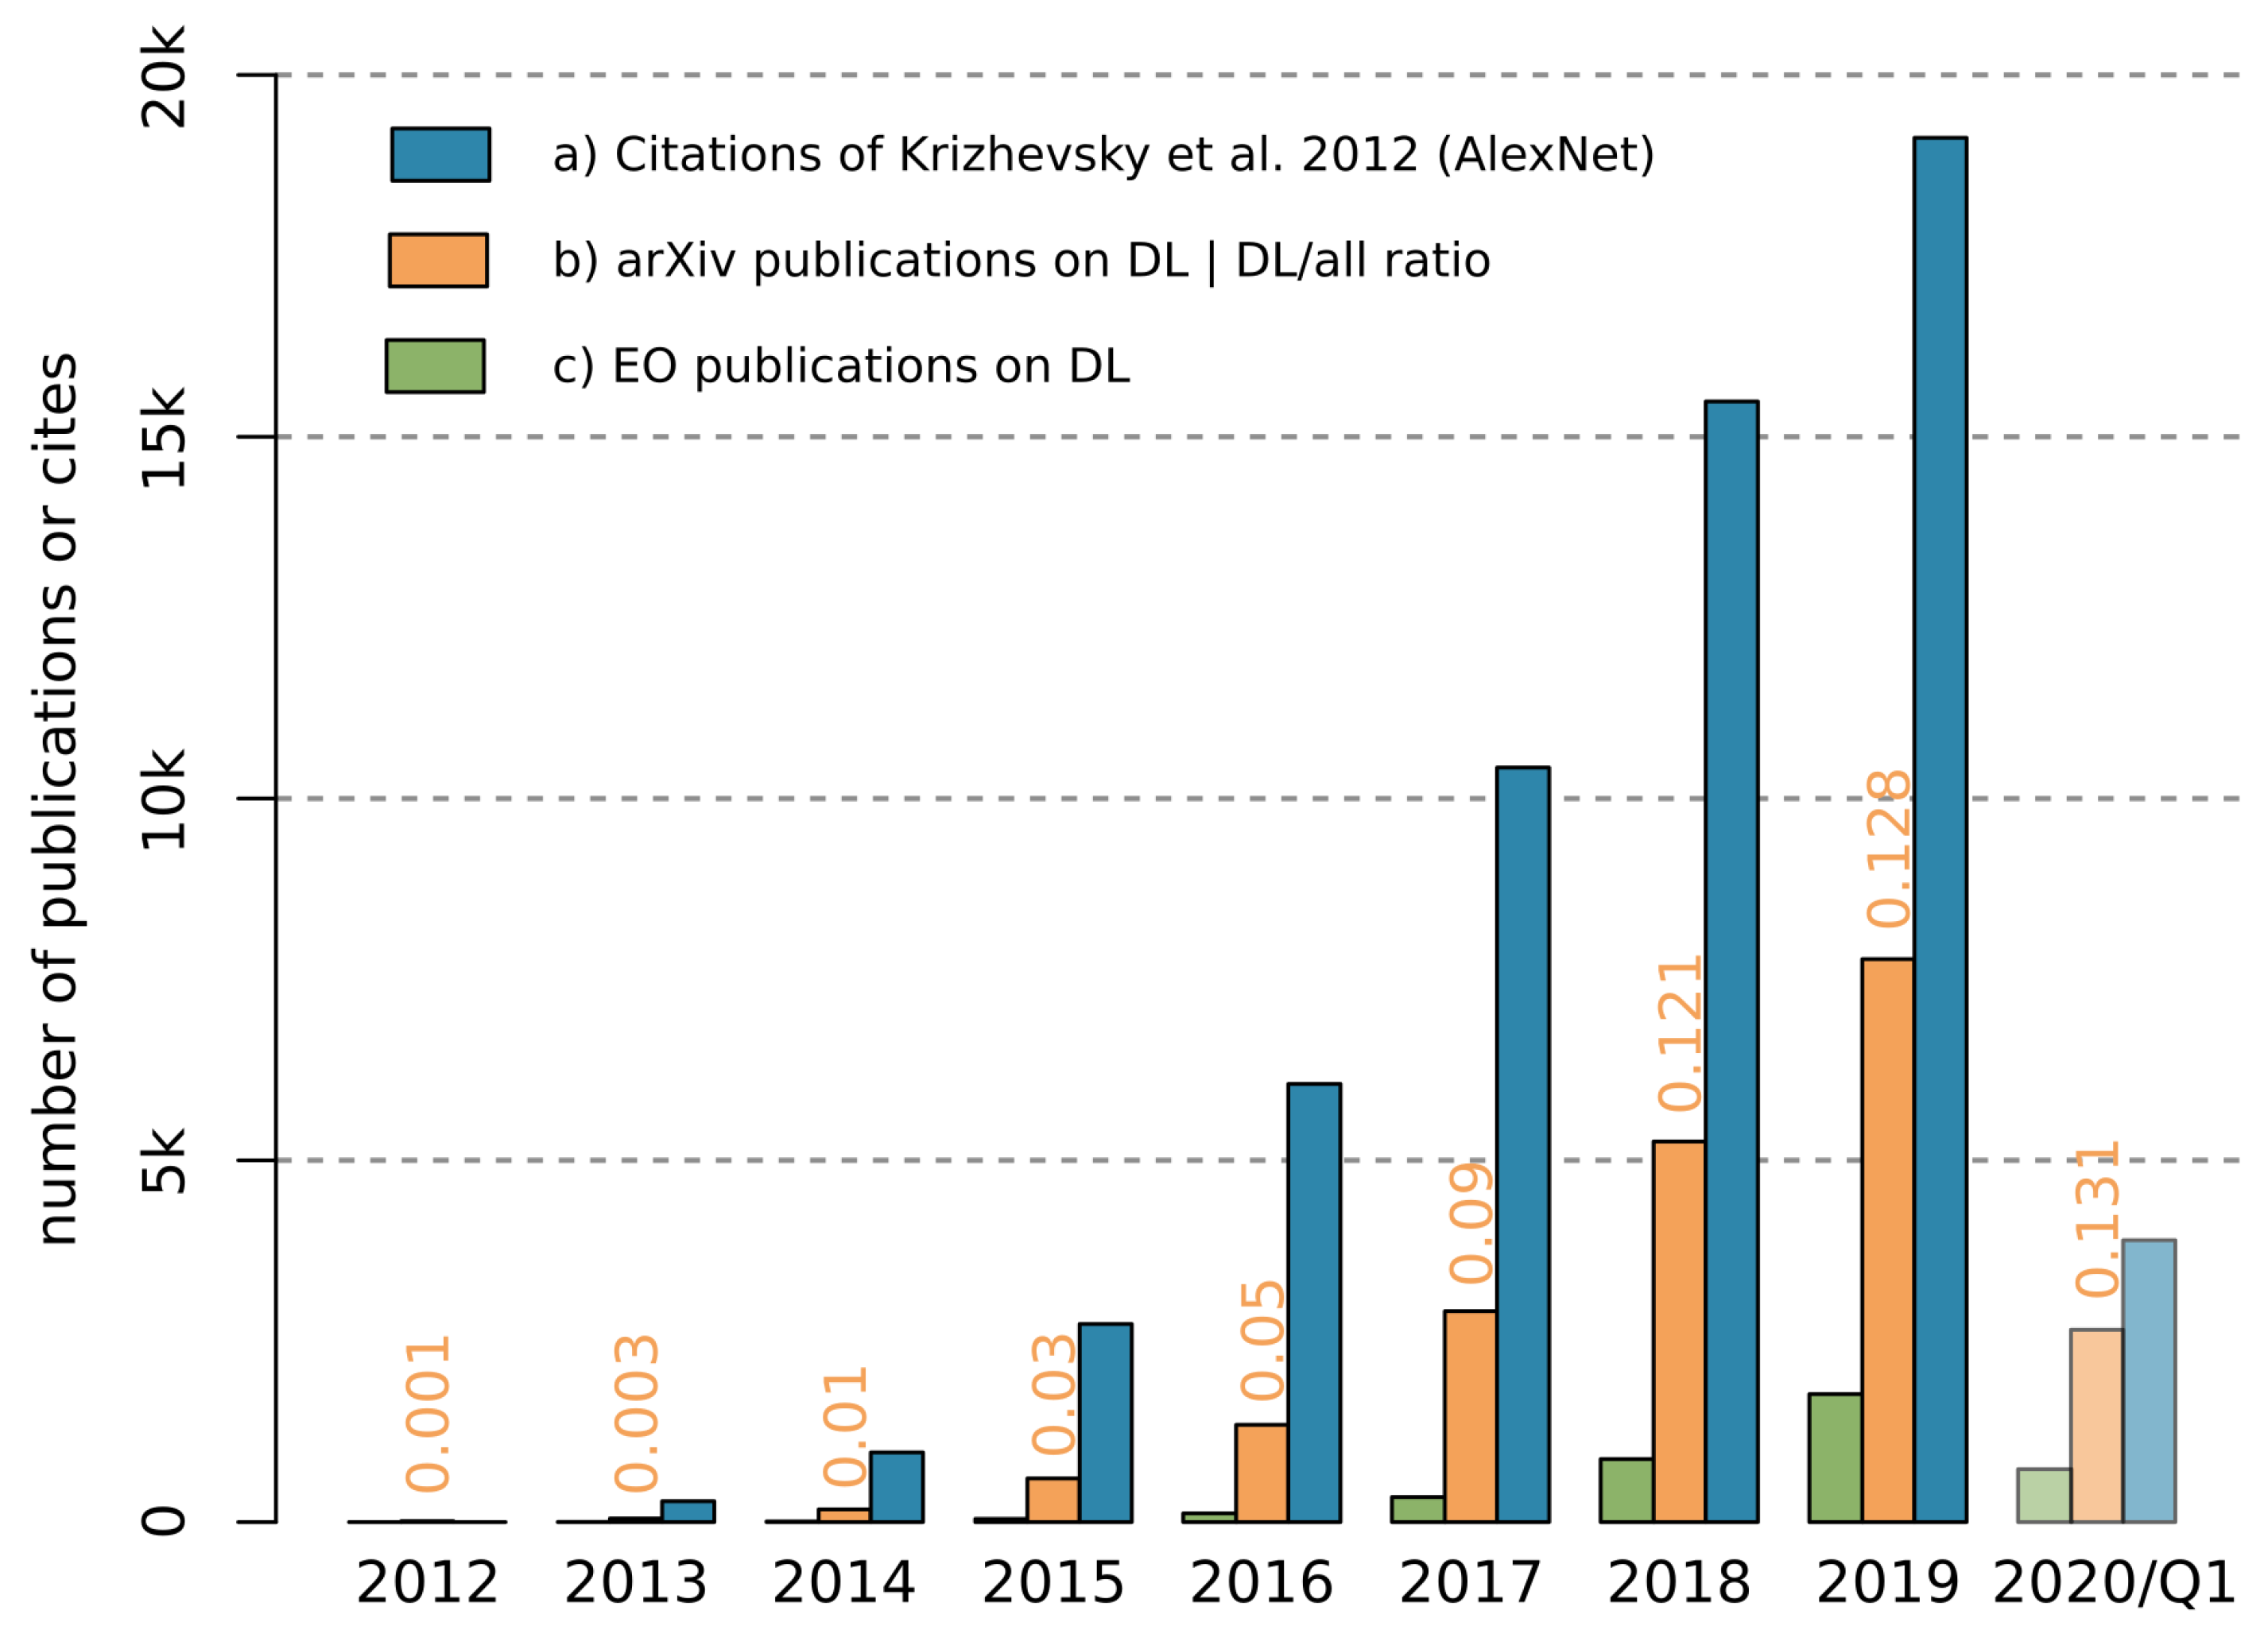
\includegraphics[width=0.6\linewidth]{./pictures/dl-papers.png}
	\caption[Papers on the use of DL]{Statistics for papers dealing with the use of deep learning in remote sensing: Citations listed in Google scholar for famous \zk{CNN} architecture \cite{cnn-classification}; arXiv listed publications in the categories \textit{cs} and \textit{stat} including the terms \textit{deep learning}, \textit{convolutional neural networks}, \textit{convolutional networks} or \textit{fully convolutional} and their share of all publications listed in the two categories; publications in selected Earth observation journals, searched for with the same terms as in arXiv, source: \cite{review-dl-eo}}
      \label{fig-dl}
\end{figure}

\begin{figure}[h]
   \centering
	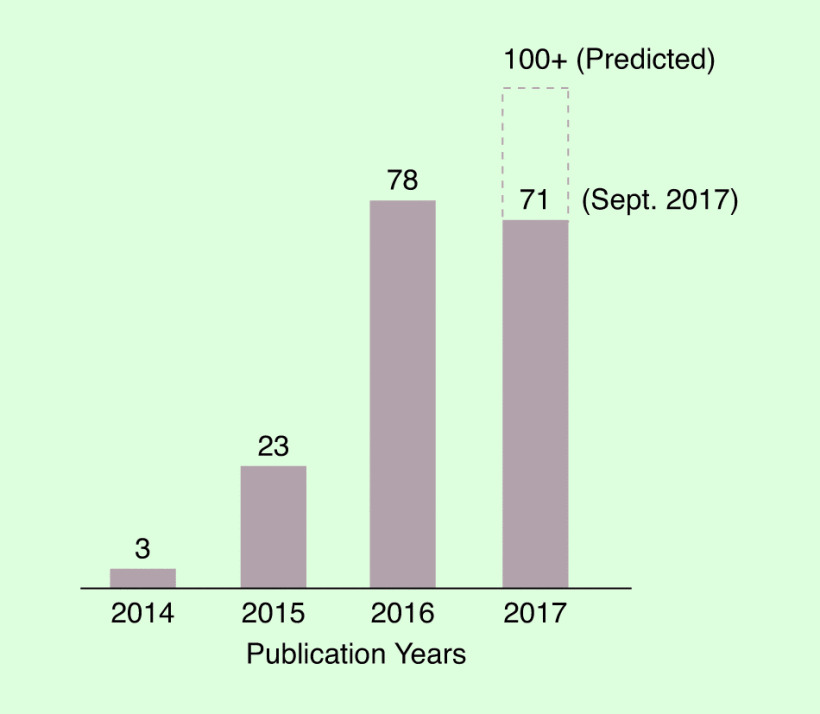
\includegraphics[width=0.6\linewidth]{./pictures/dl-rs-papers.jpg}
	\caption[Papers on the use of DL in remote sensing]{Number of papers dealing with the use of deep learning in remote sensing per year, source: \cite{review-dl-rs-2017}}
      \label{fig-rs-dl}
\end{figure}

However, this quick development of \zk{ANN}s and \zk{CNN}s makes it harder and harder for other fields as remote sensing to keep up with the progress tempo. It results in the situation where when it comes to an \zk{ANN} architecture choose, researchers without the necessary background simply choose the newest one or the one with the best reported results, although these results could be obtained on completely different data in a completely different environment and the performance could therefore very much differ from the expected one. The goal of this thesis is to try to make complex, systematic research and review of the performance of chosen \zk{CNN} architectures on various selected use cases from the field of remote sensing, and hopefully serve as a valuable guidebook when it comes to \zk{CNN} applications in the field or comparison metrics when a new architecture is proposed.

Chapter \ref{motivation} will present research on the use of comparisons when it comes to papers dealing with \zk{CNN} models in the field of remote sensing and systematically investigate their senses of comparing the original input with the already existing work from different points of view to give them sufficient scientific context. The same systematical investigation will be done also for reviews of the use of \zk{CNN}s in the field.

% TODO: Delete info about the professional debate
Chapter \ref{use-cases} will present use cases selected as test tasks to evaluate chosen architectures. For purposes of the professional debate, only one use case is presented.

These chapters will be later followed by a chapter on selected architectures and methods and a chapter presenting the results of the experiments. For purposes of the professional debate, these are not present.
\chapter{Motivation}
\label{motivation}

In August 2020, an experiment was conducted - a query for papers with the below-described restrictions was done on selected academic database websites. The goal of the experiment was to research whether authors of papers dealing with the use of convolutional neural networks (\zk{CNN}) in the field of remote sensing are comparing results of proposed or used architectures with results of other architectures on the same task. This experiment is summarized in chapter \ref{top-papers}.

This experiment was immediately followed by an overview of the top \textit{review-type} papers - as something akin is the goal of this thesis, it could be taken as the~summary of the~current situation and research on work dealing with the~same problems. This is summarized in chapter \ref{situation}.

% possible titles:
% Top cited papers dealing with use of convolutional neural networks in the field of remote sensing
\section{Articles on CNNs in the field of remote sensing}
\label{top-papers}

\subsection{Web of Science}
\label{wos-papers}

\subsubsection{Using the search term \textit{convolutional neural network}}
\label{wos-papers-full-length}

The first used website was Web of Science\footnote{\url{www.webofknowledge.com}} (\zk{WoS}). The~following query restrictions were used:

\begin{itemize}
	\item \verb|Search string: convolutional neural network|. To focus only on articles dealing with \zk{CNN}s.
	\item \verb|Search field: All Fields|. To check also articles dealing with with the topic, but not specifying it in the~title nor the abstract or keywords. This way, articles that aim more general - primarily to remote sensing or \zk{CNN}s - but dealing also with the second of the~subjects could be found.
	\item \verb|Publication years: 2020, 2019, 2018|. To focus only on recent publications.
	\item \verb|Web of Science categories: REMOTE SENSING|. To focus only on the~scien\-ti\-fic area of interest.
	\item \verb|Open Access: DOAJ Gold|. To focus only on articles and papers from sources listed on the~Di\-rectory of Open Access Journals\footnote{\url{www.doaj.org}} (\zk{DOAJ}).
\end{itemize}

\noindent The top five results from the query, when ordered by the~attribute \verb|Times Cited| and filtered as will be described below, were the following:

\begin{itemize}
	\item Building Extraction in Very High Resolution Remote Sensing Imagery Using Deep Learning and Guided Filters: 81 citations. \cite{res-u-net}
	\item Very Deep Convolutional Neural Networks for Complex Land Cover Mapping Using Multispectral Remote Sensing Imagery: 71 citations. \cite{very-deep-cnn-lc}
	\item Evaluation of Different Machine Learning Methods and Deep-Learning Convolutional Neural Networks for Landslide Detection: 51 citations. \cite{landslide-evaluation}
	\item 3D Convolutional Neural Networks for Crop Classification with Multi-Temporal Remote Sensing Images: 50 citations. \cite{3d-cnn-crop}
	\item Multi-Temporal Land Cover Classification with Sequential Recurrent Encoders: 38 citations. \cite{multi-temporal-sequential-recurrent}
\end{itemize}

\textit{Building Extraction in Very High Resolution Remote Sensing Imagery Using Deep Learning and Guided Filters} proposes a new \zk{CNN} architecture based on the residual network (\zk{ResNet}) \cite{resnet} called Res-U-Net and - using explicitly defined metrics - compares it to those of SegNet \cite{segnet}, fully convolutional network (\zk{FCN}) \cite{fcn}, a combination of \zk{CNN} and random forest (\zk{RF}) \cite{rf}, Multi-scale deep network \cite{hierarchical-labeling}, and a combination of \zk{CNN}, \zk{RF} and conditional random fields (\zk{CRF}) \cite{hierarchical-labeling}, but authors do not explain how exactly are these models built, so it does not give the~reader any solid comparison. Especially terms like \zk{CNN} and \zk{FCN} are so general that they do not imply anything more than just the basic approach. In the end, it is not even sure whether authors have tested these models on the~datasets on their own, or if they just report results found in other articles. Authors experiment on two datasets differing in used bands and spatial resolution, and also with including and excluding the normalized differential vegetation index (\zk{NDVI}) and the digital surface model (\zk{DSM}). However, both datasets are of German cities and therefore very similar in the~content, both also being binary datasets containg only two classes - \textit{building} and \textit{clutter} (unknown). Time and memory needs are not mentioned in the~study.

The second reviewed article - \textit{Very Deep Convolutional Neural Networks for Complex Land Cover Mapping Using Multispectral Remote Sensing Imagery} - deals with land cover mapping using \zk{CNN}s with a focus on wetlands detection. Therefore it is not a surprise that they do not experiment with different datasets; however, it would give much more general overview of \zk{CNN} possibilities in the wetland detection data from different parts of the world were used, and not only from Newfoundland and Labrador, Canada. Besides that, the paper experiments with DenseNet-121 \cite{densenet}, Inception V3 \cite{inception}, VGG-16 \cite{vgg}, VGG-19, Xception \cite{xception}, \zk{ResNet}-50, and Inception \zk{ResNet} V2 \cite{inception-resnet}, and also with machine learning (\zk{ML}) methods of support vector machine (\zk{SVM}) \cite{svm} and \zk{RF}. Authors also use different patch sizes and report processing times.

The third result contains the phrase \textit{evaluation of different methods} already in the title and compares \zk{CNN}s with other popular \zk{ML} methods, namely \zk{SVM}, \zk{RF}, and even with a simple artificial neural network (\zk{ANN}) architecture called multi-layer perceptron (\zk{MLP}) \cite{mlp} with a hidden layer of 30 neurons. Even the \zk{CNN} approach is diversified into two architectures - one of them comprising of five layers, the other one of seven layers. To make the results more general, authors experiment also with five different input window sizes, compare the~use of spectral bands versus the~use of a combination of spectral bands and topographical ones, and apply their models on two different datasets. Time consumption of different methods would be also valuable information on the comparison, yet this metric is not included in the article. It is apparent that authors of the paper came from the same impulse as this thesis, reading statements like \textit{"CNNs do not automatically outperform ANN, SVM and RF, although this is sometimes claimed. Rather, the performance of CNNs strongly depends on their design, i.e., layer depth, input window sizes and training strategies."} Or, in another place, \textit{"CNN will not automatically outperform other methods - as popular science articles and magazines may imply."} With felicitously set parameters, \zk{CNN}s outperformed other approaches, but their use was done under critical supervision and without trend-surfing shouts.

The fourth article, \textit{3D Convolutional Neural Networks for Crop Classification with Multi-Temporal Remote Sensing Images}, again experiments with different kernel sizes and other parameters, and compares the proposed 3D \zk{CNN} architecture with K-nearest neighbour (\zk{KNN}) \cite{knn}, principal component analysis (\zk{PCA}) \cite{pca}, \zk{SVM}, and an ad-hoc defined 2D \zk{CNN} structure. No time consumption analysis of different approaches was presented. Although the presented results seem to prove their claims that their proposed architecture performs better than the other ones, a more extensive research experimenting with more datasets and more advanced, state-of-the-art architectures could give such claims more solid position.

% The proposed method in this work can obtain improvements in terms of overall accuracy, precision and F_1 over the classical classification systems.

Authors of \textit{Multi-Temporal Land Cover Classification with Sequential Recurrent Encoders} do admit that their comparison part is not ideal; that is true as they compare results of their proposed architecture only with results of other architectures reported in other papers - these results were achieved using different datasets, different preprocessing, different numbers of classes and training samples, different spatial resolution and different bands. Therefore, it is arguable whether this comparison is relevant at all. Authors test their architecture on a multi-class dataset coming from one area in Germany split into two years; this also does not serve as a test on multiple independent datasets. Positive is the~fact that authors explicitly define used quality metrics and report time needs of the training, although only the~overall accuracy is presented for other architectures in the~comparison table.

Using the same query, but restrictive to search only in the topic (searching the title, the abstract, and keywords), the results were the same.

\subsubsection{Using the search term \textit{cnn}}
\label{wos-papers-cnn}

As in some articles, only the abbreviation \textit{\zk{CNN}} is used instead of the full-length term \textit{convolutional neural network}, the~same research using \textit{\zk{CNN}} as the search term was done.

\begin{itemize}
	\item \verb|Search string: cnn|. To focus only on articles dealing with \zk{CNN}s.
	\item \verb|Search field: All Fields|. To check also articles dealing with with the topic, but not specifying it in the~title nor the abstract or keywords. This way, articles that aim more general - primarily to remote sensing or \zk{CNN}s - but dealing also with the second of the~subjects could be found.
	\item \verb|Publication years: 2020, 2019, 2018|. To focus only on recent publications.
	\item \verb|Web of Science categories: REMOTE SENSING|. To focus only on the~scien\-ti\-fic area of interest.
	\item \verb|Open Access: DOAJ Gold|. To focus only on articles and papers from sources listed on the~Di\-rectory of Open Access Journals\footnote{\url{www.doaj.org}} (\zk{DOAJ}).
\end{itemize}

\noindent The top five results from the query, when ordered by the~attribute \verb|Times Cited| and filtered as will be described below, were the following:

\begin{itemize}
	\item Evaluation of Different Machine Learning Methods and Deep-Learning Convolutional Neural Networks for Landslide Detection: 51 citations. \cite{landslide-evaluation}
	\item 3D Convolutional Neural Networks for Crop Classification with Multi-Temporal Remote Sensing Images: 50 citations. \cite{3d-cnn-crop}
	\item Geospatial Object Detection in High Resolution Satellite Images Based on Multi-Scale Convolutional Neural Network: 32 citations. \cite{object-detection-hrs-multi-scale}
	\item Hyperspectral Image Classification Using Convolutional Neural Networks and Multiple Feature Learning: 31 citations. \cite{hyperspectral-multiple-feat-cnn}
	\item Deformable Faster R-CNN with Aggregating Multi-Layer Features for Partially Occluded Object Detection in Optical Remote Sensing Images: 24 citations. \cite{deformable-faster-r-cnn}
\end{itemize}

Two results were filtered out. \cite{cnn-fusion-clouds} with 28 citations and \cite{cnn-fusion-hr-hsr} with 25 citations. They were filtered out only because they do not correspond with the~main focus of the~thesis on the classification task with object detection and semantic and instance segmentation, but dealt with an image fusion instead. The top two results correspond to articles reviewed already in the previous section; therefore they are being skipped now.

The comparison part of \textit{Geospatial Object Detection in High Resolution Satellite Images Based on Multi-Scale Convolutional Neural Network} is a bit more minimalistic. The proposed method is compared only with an architecture called Faster \zk{R-CNN} (region based convolutional neural network) \cite{faster-rcnn} and with the single shot multi-box detector (\zk{SSD}) \cite{ssd} without a more detailed description of inner parametrization or experiments with it. Authors use also only one dataset to test their method, so there is no evidence on how versatile the method is when it comes to the data greed. On the other hand, they report the time greed of the three used methods.

In \textit{Hyperspectral Image Classification Using Convolutional Neural Networks and Multiple Feature Learning}, authors go a~different way - to compare their architecture, they create two different architectures and show that the~proposed one is the~one performing the best. A comparison with any other well-known architecture or other \zk{ML} method is missing. The pro of this paper is the use of three different datasets.

24 citations reaching \textit{Deformable Faster R-CNN with Aggregating Multi-Layer Features for Partially Occluded Object Detection in Optical Remote Sensing Images} also proposes a new architecture, called \textit{deformable R-CNN}. Authors compare this model with \zk{SSD} and R-P-Faster \zk{R-CNN} \cite{rp-faster-rcnn} on three datasets. No comparison of time or memory requirements is included in the article.

Using the same query, but restrictive to search only in the topic (searching the title, the abstract, and keywords), the results were the same.

% Convolution Neural Network Architecture Learning for Remote Sensing Scene Classification
% https://arxiv.org/abs/2001.09614

% Murthy, C.; Raju, P.; Badrinath, K. Classification of wheat crop with multi-temporal images: Performance of maximum likelihood and artificial neural networks. Int. J. Remote Sens. 2003, 24, 4871–4890. ?????????????????????????????

% Lin, H.; Shi, Z.; Zou, Z. Maritime Semantic Labeling of Optical Remote Sensing Images with Multi-Scale Fully Convolutional Network. ????????????

% WoS #2
% Geospatial Object Detection in High Resolution Satellite Images Based on Multi-Scale Convolutional Neural Network
% https://apps.webofknowledge.com/full_record.do?product=WOS&search_mode=GeneralSearch&qid=8&SID=C6dRsuZprCvu65HT7SF&page=1&doc=2&cacheurlFromRightClick=no
% superiority of the proposed method

% #3
% superior performances of the proposed framework

% #4
% Deformable Faster R-CNN with Aggregating Multi-Layer Features for Partially Occluded Object Detection in Optical Remote Sensing Images
% https://apps.webofknowledge.com/full_record.do?product=WOS&search_mode=GeneralSearch&qid=5&SID=C6pjuytIsVIIBFmwnOt&page=1&doc=4&cacheurlFromRightClick=no
% compared with SSD, R-P-Faster R-CNN, also compared on three datasets (NWPU, SORSI, HRRS), no comparison on time or memory usage

% #5
% Ship Detection Based on YOLOv2 for SAR Imagery
% https://apps.webofknowledge.com/full_record.do?product=WOS&search_mode=GeneralSearch&qid=5&SID=C6pjuytIsVIIBFmwnOt&page=1&doc=5&cacheurlFromRightClick=no
% compared with Faster R-CNN and not with YOLOv2 or YOLO, two datasets (both about ships), compared time needs
% "YOLOv2-reduced is best for real time object detection problem."

\subsection{Scopus}
\label{scopus-papers}

\subsubsection{Using the search term \textit{convolutional neural network}}
\label{scopus-papers-full-length}

The second used website was Scopus\footnote{\url{www.scopus.com}}. The~following query restrictions were used:

\begin{itemize}
	\item \verb|Search string: "remote sensing" "convolutional neural network"|. To focus only on articles dealing with \zk{CNN}s in the area of remote sensing.
	\item \verb|Search field: All fields|. To check also articles dealing with with the topic, but not specifying it in the~title nor the abstract or keywords. This way, articles that aim more general - primarily to remote sensing or \zk{CNN}s - but dealing also with the second of the~subjects could be found.
	\item \verb|Publication years: 2020, 2019, 2018|. To focus only on recent publications.
	\item \verb|Access type: Open Access|. To focus only on articles in \textit{Scopus Gold Open Access}\footnote{\url{www.elsevier.com/open-access}}. It includes fully open journals, hybrid journals (authors pay a fee to make an article open access), open archives and articles with free promotional access.
\end{itemize}

\noindent The Scopus query is apparently - probably due to the~smaller flexibility when it comes to the~open access restrictions - more tolerant and includes articles filtered out from the~\zk{WoS} query. Also, because there is no scientific category \verb|remote sensing| in the~Scopus search engine, the~phrase was included in the~search phrase and more manual filtering was needed, as will be described below. The~top five results from the query, when ordered by the~attribute \verb|Cited by|, were the following:

\begin{itemize}
	\item A new deep convolutional neural network for fast hyperspectral image classification: 123 citations.  \cite{cnn-hs-class}
	\item Automatic ship detection in remote sensing images from google earth of complex scenes based on multiscale rotation Dense Feature Pyramid Networks: 97 citations. \cite{ship-rdfpn}
	\item Deep learning in remote sensing applications: A meta-analysis and review: 93 citations. \cite{dl-remote-sensing-review}
	\item Building extraction in very high resolution remote sensing imagery using deep learning and guided filters: 92 citations. \cite{res-u-net}
	\item Semi-Supervised Deep Learning Using Pseudo Labels for Hyperspectral Image Classification: 77 citations \cite{semi-supervised-hyperspectral}
\end{itemize}

Ten results were filtered out. \cite{dl-for-cv} with 251 citations, \cite{ir-image-fusion} with 200 citations, \cite{review-ml-in-rs} with 177 citations, \cite{rf-knn-svm-for-lc} with 157 citations, \cite{review-ml-agriculture} with 153 citations, \cite{review-uav-applications} with 104 citations, \cite{review-survey-dl} with 98 citations, \cite{dl-medicine-preprocessing} with 87 citations, \cite{state-of-the-art-ann} with 85 citations, and \cite{lc-2-0} with 83 citations. They were filtered out only because they do not correspond with the~main focus of the~thesis on the classification task with object detection and semantic and instance segmentation in the field of remote sensing.

The first article, \textit{A new deep convolutional neural network for fast hyperspectral image classification}, starts the~research again in a very positive way. Authors have compared their own architecture with the \zk{MLP} and three different \zk{CNN}s - a one-dimensional one, a two-dimensional one and a three-dimensional one. Although a~comparison with some popular architectures that just haven't been used on hyperspectral images or some classical \zk{ML} methods would be also interesting, the used ones are properly sourced to another research on hyperspectral image classification and authors underlined main differences between the proposed model and the ones used for evaluation. All experiments have been conducted on two datasets differing in the number of bands, pixel size of images, spatial resolution, and also in objects of classification. Authors also experiment with different patch sizes and - importantly - with the~number of samples per class.

\textit{Automatic ship detection in remote sensing images from google earth of complex scenes based on multiscale rotation Dense Feature Pyramid Networks} also does not compare the~proposed methodology with basic \zk{ML} approaches, but uses a lot of \zk{CNN} models to compare their architecture with - Faster \zk{R-CNN}, Feature pyramid network (\zk{FPN}) \cite{fpn}, rotation region proposal network (\zk{RRPN}) \cite{rrpn}, and rotational region convolutional neural network (\zk{R2CNN}) \cite{r2cnn}. However, as the~paper focuses only on the~ship detection, there is no experiment on other datasets.

The third most cited article on Scopus - \textit{Deep learning in remote sensing applications: A meta-analysis and review} - is a review coming from similar impulses as this thesis or partly \cite{landslide-evaluation} mentioned in chapter \ref{wos-papers}. The motivation is formulated in the sense that \textit{"it appears that a more systematic (i.e. quantitative) analysis is necessary to get a comprehensive and objective understanding of the applications of DL for remote-sensing analysis."}. Authors focus on many more fields than is the goal of this thesis, including image fusion, image registration, scene classification, object detection, land use and land cover classification, image segmentation, object-based image analysis (\zk{OBIA}), and other tasks. The~value of the~paper lies in its extensive research on what are the~most frequent targets of the~use of deep learning (\zk{DL}) for remote sensing, what are the~most frequent \zk{DL} models, spatial resolutions, application areas (urban, vegetation, etc.), average accuracies, common training datasets and even the~most used scientific terms in titles and abstracts of these papers. Although it is a high-class review and it works as a valuable overview about \zk{DL} stronger and weaker positions in the~field, authors have not conducted their own experiments, so only results reported in the~original papers are mentioned, if mentioned.

\textit{Building extraction in very high resolution remote sensing imagery using deep learning and guided filters} is the same one as the one mentioned in chapter \ref{wos-papers}, only with different number of citations due to the difference between the \zk{WoS} and Scopus systems; therefore it is being skipped in this section.

Authors of \textit{Semi-Supervised Deep Learning Using Pseudo Labels for Hyperspectral Image Classification} propose their own method called semi-supervised deep learning using pseudo-labels (\zk{PL-SSDL}) using convolutional recurrent neural networks (\zk{CRNN}) and compare its performace on three multi-class hyperspectral datasets differing in number of classes, number of bands, and also in the~spatial resolution (ranging from 1 metre to 2.5 metres). \zk{PL-SSDL} is compared with big amount of \zk{ML} methods, namely \zk{KNN}, \zk{SVM}, label propagation \cite{label-prop}, transductive support vector machine (\zk{TSVM}) \cite{tsvm}, Laplacian support vector machine (\zk{LapSVM}) \cite{lapsvm}, and spatio-spectral Laplacian support vector machine (\zk{SS-LapSVM}) \cite{ss-lapsvm}, and two \zk{ANN} architectures, namely stacked denoising autoencoder (\zk{SDA}) \cite{sda}, and ladder networks \cite{ladder-networks}. As \zk{PL-SSDL} is a \zk{CRNN}, a comparison with \zk{CNN} or \zk{RNN} or their combination would be desirable, especially considering the fact that the used \zk{ANN} models could be built using them. Authors report for every method time complexity and accuracy , but do not specify explicitly what accuracy metric do they use or how do they measure the time complexity (number of epochs is slightly mentioned for \zk{PL-SSDL}, but not for any other approach).

Using the same query, but restrictive to search only in the title, the abstract, and keywords, the results were as follows:

\begin{itemize}
	\item A new deep convolutional neural network for fast hyperspectral image classification: 123 citations.  \cite{cnn-hs-class}
	\item Semi-Supervised Deep Learning Using Pseudo Labels for Hyperspectral Image Classification: 77 citations \cite{semi-supervised-hyperspectral}
	\item Very Deep Convolutional Neural Networks for Complex Land Cover Mapping Using Multispectral Remote Sensing Imagery: 72 citations. \cite{very-deep-cnn-lc}
	\item 3D Convolutional Neural Networks for Crop Classification with Multi-Temporal Remote Sensing Images: 61 citations. \cite{3d-cnn-crop}
	\item Hyperspectral Image Classification Using Convolutional Neural Networks and Multiple Feature Learning: 54 citations. \cite{hyperspectral-multiple-feat-cnn}
\end{itemize}

From the~results above, the two top articles were already received with the \verb|All Fields| query. The rest was reviewed already in chapter \ref{wos-papers}, only with different number of citations due to the difference between the \zk{WoS} and Scopus systems. Therefore, all of them are being skipped now.

\subsubsection{Using the search term \textit{cnn}}
\label{scopus-papers-cnn}

As in some articles, only the abbreviation \textit{\zk{CNN}} is used instead of the full-length term \textit{convolutional neural network}, the~same research using \textit{\zk{CNN}} as the search term was done.

\begin{itemize}
	\item \verb|Search string: "remote sensing" cnn|. To focus only on articles dealing with \zk{CNN}s in the area of remote sensing.
	\item \verb|Search field: All fields|. To check also articles dealing with with the topic, but not specifying it in the~title nor the abstract or keywords. This way, articles that aim more general - primarily to remote sensing or \zk{CNN}s - but dealing also with the second of the~subjects could be found.
	\item \verb|Publication years: 2020, 2019, 2018|. To focus only on recent publications.
	\item \verb|Access type: Open Access|. To focus only on articles in \textit{Scopus Gold Open Access}\footnote{\url{www.elsevier.com/open-access}}. It includes fully open journals, hybrid journals (authors pay a fee to make an article open access), open archives and articles with free promotional access.
\end{itemize}

\noindent The Scopus query is apparently - due to the~smaller flexibility when it comes to the~open access restrictions - more tolerant and includes articles filtered out from the~\zk{WoS} query. Also, because there is no scientific category \verb|remote sensing| in the~Scopus search engine, the~phrase was included in the~search phrase and more manual filtering was needed, as will be described below. The~top five results from the query, when ordered by the~attribute \verb|Cited by|, were the following:

\begin{itemize}
	\item A new deep convolutional neural network for fast hyperspectral image classification: 123 citations.  \cite{cnn-hs-class}
	\item Automatic ship detection in remote sensing images from google earth of complex scenes based on multiscale rotation Dense Feature Pyramid Networks: 97 citations. \cite{ship-rdfpn}
	\item Deep learning in remote sensing applications: A meta-analysis and review: 93 citations. \cite{dl-remote-sensing-review}
	\item Building extraction in very high resolution remote sensing imagery using deep learning and guided filters: 92 citations. \cite{res-u-net}
	\item Very Deep Convolutional Neural Networks for Complex Land Cover Mapping Using Multispectral Remote Sensing Imagery: 72 citations. \cite{very-deep-cnn-lc}
\end{itemize}

Four results were filtered out. \cite{dl-for-cv} with 251 citations, \cite{dl-lungs} with 87 citations, \cite{maoxian-landslide} with 74 citations, and \cite{state-of-the-art-dl} with 73 citations. They were filtered out only because they do not correspond with the~main focus of the~thesis on the classification task with object detection and semantic and instance segmentation in the field of remote sensing.

From the~results above, the top four results correspond to articles reviewed already in the previous section and the fifth one to an article reviewed already in chapter \ref{wos-papers}, only with different number of citations due to the difference between the \zk{WoS} and Scopus systems. Therefore, all of them are being skipped in this section.

Using the same query, but restrictive to search only in the title, the abstract, and keywords, the results were as follows:

\begin{itemize}
	\item A new deep convolutional neural network for fast hyperspectral image classification: 123 citations.  \cite{cnn-hs-class}
	\item Very Deep Convolutional Neural Networks for Complex Land Cover Mapping Using Multispectral Remote Sensing Imagery: 72 citations. \cite{very-deep-cnn-lc}
	\item 3D Convolutional Neural Networks for Crop Classification with Multi-Temporal Remote Sensing Images: 61 citations. \cite{3d-cnn-crop}
	\item Small object detection in optical remote sensing images via modified Faster R-CNN: 57 citations. \cite{modified-faster-rcnn-small-objects}
	\item Hyperspectral Image Classification Using Convolutional Neural Networks and Multiple Feature Learning: 54 citations. \cite{hyperspectral-multiple-feat-cnn}
\end{itemize}

From the~results above, the two top results correspond to articles reviewed already in the previous section and the third and fifth one to articles reviewed already in chapter \ref{wos-papers}, only with different number of citations due to the difference between the \zk{WoS} and Scopus systems. Therefore, only the fourth one is being reviewed in this section.

\textit{Small object detection in optical remote sensing images via modified Faster R-CNN} proposes a modified Faster \zk{R-CNN}-based architecture and tries it on the task of the aeroplanes and ships detection. The goal of the paper is to show that the proposed architecture improves the performance of the baseline Faster \zk{R-CNN}, so the comparison with the original model is not surprising, although showing a relative comparison with some other architectures to show the full picture would be valuable; even the Faster \zk{R-CNN}-modified Faster \zk{R-CNN} comparison is a bit vague as variable parameters that affect the performance of the architecture like the backbone architecture and the total stride are defined differently for each case in the presented experiment. A test on a different dataset or a task would be also beneficial, as well as info about the time needs of the new model.

\section{Reviews of CNNs in the field of remote sensing}
\label{situation}

\subsection{Web of Science}
\label{wos-reviews}

\subsubsection{Using the search term \textit{convolutional neural network}}
\label{wos-reviews-full-length}

When compared with the query described in chapter \ref{wos-papers}, an extra parameter \verb|Document Types| was used to get only \textit{review-type} articles. Therefore, the following restrictions were used for the~query:

\begin{itemize}
	\item \verb|Search string: convolutional neural network|. To focus only on articles dealing with \zk{CNN}s.
	\item \verb|Search field: All Fields|. To check also articles dealing with with the topic, but not specifying it in the~title nor the abstract or keywords. This way, articles that aim more general - primarily to remote sensing or \zk{CNN}s - but dealing also with the second of the~subjects could be found.
	\item \verb|Publication years: 2020, 2019, 2018|. To focus only on recent publications.
	\item \verb|Web of Science categories: REMOTE SENSING|. To focus only on the~scien\-ti\-fic area of interest.
	\item \verb|Open Access: DOAJ Gold|. To focus only on articles and papers from sources listed on the~Di\-rectory of Open Access Journals\footnote{\url{www.doaj.org}} (\zk{DOAJ}).
	\item \verb|Document Types: REVIEW|. To focus only on reviews.
\end{itemize}

\noindent There were only seven results for the~described query and two of them - \textit{Spatiotemporal Image Fusion in Remote Sensing} \cite{review-st-fusion} with 14 citations and \textit{Meta-Analysis of Wetland Classification Using Remote Sensing: A Systematic Review of a 40-Year Trend in North America} \cite{review-wetlands-40-years} with 0 citations - were filtered out as they dealt with the~image fusion and with the history of wetland classification and did not overlay with the main focus of this thesis. The rest, when ordered by the~attribute \verb|Times Cited|, were the following:

\begin{itemize}
	\item Review and Evaluation of Deep Learning Architectures for Efficient Land Cover Mapping with UAS Hyper-Spatial Imagery: A Case Study Over a Wetland: 3 citations. \cite{review-dl-wetlands}
	\item Object Detection and Image Segmentation with Deep Learning on Earth Observation Data: A Review-Part I: Evolution and Recent Trends: 1 citation. \cite{review-dl-eo}
	\item Geographic Object-Based Image Analysis: A Primer and Future Directions: 0 citations. \cite{geobia}
	\item Deep Learning for Land Use and Land Cover Classification Based on Hyperspectral and Multispectral Earth Observation Data: A Review: 0 citations. \cite{review-dl-lulc}
	\item Deep Learning Approaches Applied to Remote Sensing Datasets for Road Extraction: A State-Of-The-Art Review: 0 citations. \cite{review-dl-road-extraction}
\end{itemize}

As \cite{very-deep-cnn-lc}, \textit{Review and Evaluation of Deep Learning Architectures for Efficient Land Cover Mapping with UAS Hyper-Spatial Imagery: A Case Study Over a Wetland} focuses on wetlands. And although authors evaluate and describe a pleasurable amount of architectures including SegNet, U-Net \cite{u-net}, DenseNet, DeepLab V3+ \cite{deeplab}, Pyramid scene parsing network (\zk{PSPNet}) \cite{pspnet}, and an architecture called MobileU-Net (a combination of MobileNet \cite{mobilenet} and U-Net) and dedicate a lot of space to used evaluation metrics, their findings would be even more valuable and universal if tested on more than one dataset. An application of at least one of the~common \zk{ML} methods would also give the~article an added value in the form of a~well-understood relative comparison.

\textit{Object Detection and Image Segmentation with Deep Learning on Earth Observation Data: A Review-Part I} (part two is as of August 14, 2020 not yet published) focuses on an overview and the~evolution of different approaches in the topic. Authors present a comprehensive overview of \zk{DL} architectures commonly or less commonly used on Earth observation (\zk{EO}) data, but - due to their main goal being just an overview - do not conduct their own experiments; instead, they report results based on the~\zk{MS-COCO} dataset (Microsoft-Common Objects in Context) \cite{coco}, a dataset with contents very different than those of \zk{EO} data.

The main focus of \textit{Geographic Object-Based Image Analysis: A Primer and Future Directions} is on the geographic object-based analysis (\zk{GEOBIA}) and not \zk{CNN}s; however, a not negligible part of the~review deals with \zk{CNN}s and \zk{CNN}s - called geographic object-based convolutional neural networks (\zk{GEOCNN}s) - are proposed as one of the~most promising future directions of \zk{GEOBIA}. But when it comes to the~chapter \textit{Accuracies of GEOCNN Methods Versus Conventional GEOBIA}, no experiments are conducted and the~entire report is reduced to citations with trifling claims without numbers like \textit{"method following Approach 3 resulted in higher thematic accuracy than per-pixel classification with patch-based CNNs and FCNs"} or \textit{"method following Approach 2 resulted in higher segmentation accuracy than GEOBIA"}.

As in \cite{review-dl-eo}, authors of \textit{Deep Learning for Land Use and Land Cover Classification Based on Hyperspectral and Multispectral Earth Observation Data: A Review} also do not conduct any experiment, but rather report the evolution of the \zk{DL} and land cover and land use classification. And although they sketch the connection between different topic problems and different \zk{ML} or \zk{DL} architectures, they do not report any numbers and when they rarely write about about performances, only general phrases like \textit{"U-Net has shown very promising results in extracting buildings"} are used.

\textit{Deep Learning Approaches Applied to Remote Sensing Datasets for Road Extraction: A State-Of-The-Art Review} introduces different approaches to road extraction using \zk{DL}. Although it gives always multiple model examples for every approach, their results - crucial for the right model choice - are taken from original papers; therefore, different metrics are used, time needs are mentioned only exceptionally, and different datasets are used, and even when the same dataset is used, different setting (as the training-validation images ratio) could lead to different scores.

Using the same query, but restrictive to search only in the topic (searching the title, the abstract, and keywords), the results were the same.

\subsubsection{Using the search term \textit{cnn}}
\label{wos-reviews-cnn}

As in some articles, only the abbreviation \textit{\zk{CNN}} is used instead of the full-length term \textit{convolutional neural network}, the~same research using \textit{\zk{CNN}} as the search term was done.

\begin{itemize}
	\item \verb|Search string: cnn|. To focus only on articles dealing with \zk{CNN}s. The~term \verb|cnn| was preferred over the~term \verb|convolutional neural network| as in some papers, only the~abbreviated form was used (this does not apply to papers only marginally mentioning \zk{CNN}s, where the term is normally full-length).
	\item \verb|Search field: All Fields|. To check also articles dealing with with the topic, but not specifying it in the~title nor the abstract or keywords. This way, articles that aim more general - primarily to remote sensing or \zk{CNN}s - but dealing also with the second of the~subjects could be found.
	\item \verb|Publication years: 2020, 2019, 2018|. To focus only on recent publications.
	\item \verb|Web of Science categories: REMOTE SENSING|. To focus only on the~scien\-ti\-fic area of interest.
	\item \verb|Open Access: DOAJ Gold|. To focus only on articles and papers from sources listed on the~Di\-rectory of Open Access Journals\footnote{\url{www.doaj.org}} (\zk{DOAJ}).
	\item \verb|Document Types: REVIEW|. To focus only on reviews.
\end{itemize}

\noindent There were only five results for the~described query and one of them - \textit{Spatiotemporal Image Fusion in Remote Sensing} \cite{review-st-fusion} with 14 citations - was filtered out as it dealt with the~image fusion and not with the~classification. The rest, when ordered by the~attribute \verb|Times Cited|, were the following:

\begin{itemize}
	\item Review and Evaluation of Deep Learning Architectures for Efficient Land Cover Mapping with UAS Hyper-Spatial Imagery: A Case Study Over a Wetland: 3 citations. \cite{review-dl-wetlands}
	\item UAV-Based Structural Damage Mapping: A Review: 3 citations. \cite{uav-building-damages}
	\item Object Detection and Image Segmentation with Deep Learning on Earth Observation Data: A Review-Part I: Evolution and Recent Trends: 1 citation. \cite{review-dl-eo}
	\item Geographic Object-Based Image Analysis: A Primer and Future Directions: 0 citation. \cite{geobia}
\end{itemize}

The only review not described in the previous section is the second one. \textit{UAV-Based Structural Damage Mapping: A Review} does not focus primarily on \zk{CNN}s, but as they constitute a big part of UAV-based damage mapping, there is a lot of reviewing of them in the~article. However, the~article works more as an overview of the evolution of different approaches in the topic. Therefore, no novel experiments were conducted and when some results are mentioned, they are only copied from original papers; papers, where these methods could have been used on different data with different results.

Using the same query, but restrictive to search only in the topic (searching the title, the abstract, and keywords), the results were the same.

\subsection{Scopus}
\label{scopus-reviews}

\subsubsection{Using the search term \textit{convolutional neural network}}
\label{scopus-reviews-full-length}

When compared with the query described in chapter \ref{scopus-papers}, an extra parameter \verb|Document type| was used to get only \textit{review-type} articles. Therefore, the following restrictions were used for the~query:

\begin{itemize}
	\item \verb|Search string: "remote sensing" "convolutional neural network"|. To focus only on articles dealing with \zk{CNN}s in the area of remote sensing.
	\item \verb|Search field: All fields|. To check also articles dealing with with the topic, but not specifying it in the~title nor the abstract or keywords. This way, articles that aim more general - primarily to remote sensing or \zk{CNN}s - but dealing also with the second of the~subjects could be found.
	\item \verb|Publication years: 2020, 2019, 2018|. To focus only on recent publications.
	\item \verb|Access type: Open Access|. To focus only on articles in \textit{Scopus Gold Open Access}\footnote{\url{www.elsevier.com/open-access}}. It includes fully open journals, hybrid journals (authors pay a fee to make an article open access), open archives and articles with free promotional access.
	\item \verb|Document type: Review|. To focus only on reviews.
\end{itemize}

The Scopus query is apparently - due to the~smaller flexibility when it comes to the~open access restrictions - more tolerant and includes articles filtered out from the~\zk{WoS} query. Also, because there is no scientific category \verb|remote sensing| in the~Scopus search engine, the~phrase was included in the~search phrase. It resulted in the~fact that from the~top 20 articles when orded by the~attribute \verb|Cited by|, 19 were filtered out as they either did not correspond with the~main focus of the~thesis on the classification task with object detection and semantic and instance segmentation in the field of remote sensing, or they were found completely insufficient in terms of providing a~comparison of mentioned architectures.

The 19 filtered articles were the following: \cite{dl-for-cv} with 251 citations, \cite{review-ml-in-rs} with 177 citations, \cite{review-ml-agriculture} with 153 citations, \cite{review-uav-applications} with 104 citations, \cite{state-of-the-art-ann} with 85 citations, \cite{lc-2-0} with 83 citations, \cite{state-of-the-art-dl} with 73 citations, \cite{review-water-dl} with 71 citations, \cite{review-plant-stress} with 66 citations, \cite{review-text-class} with 53 citations, \cite{cv-animal-ecology} with 50 citations, \cite{review-cv-infra-inspections} with 49 citations, \cite{review-ann-plant-disease} with 48 citations, \cite{review-st-fusion-multisource} with 48 citations, \cite{review-ml-energy} with 47 citations, \cite{review-bd-disaster} with 43 citations, \cite{review-uav-rs} with 34 citations, \cite{nanophotonics} with 33 citations, and \cite{review-point-clouds} with 33 citations.

The only one corresponding with the aim of this thesis is \textit{Deep learning for remote sensing image classification: A survey} \cite{review-dl-rs} with 45 citations. The approach is very fulfilling - authors compare multiple architectures on multiple datasets and define metrics used for the comparison. The fact that almost half of the presented results are taken from a different source is not a problem, but the fact that in the other part, a different training-validation-test data ratio was used for different models is. Also, the researched architectures are just vaguely defined without specifying parameters used to build them.

Using the same query, but restrictive to search only in the title, the abstract, and keywords, the results were as follows:

\begin{itemize}
	\item Deep learning for remote sensing image classification: A survey: 45 citations. \cite{review-dl-rs}
	\item Hyperspectral image classification based on spectral and spatial information using multi-scale ResNet: 1 citation. \cite{hs-multi-scale-resnet}
	\item Deep Learning for Land Use and Land Cover Classification Based on Hyperspectral and Multispectral Earth Observation Data: A Review: 0 citations. \cite{review-dl-lulc}
	\item Geographic Object-Based Image Analysis: A Primer and Future Directions: 0 citations. \cite{geobia}
\end{itemize}

\noindent There were only eight results for the~described query and four of them were filtered out - \cite{review-st-fusion} with 15 citations, \cite{ml-cv-phenotyping} with 11 citations, \cite{survey-dl-rs-enhancement} with 8 citations, and \cite{survey-dl-super-resolution} with 6 citations. They were filtered out only because they do not correspond with the~main focus of the~thesis on the classification task with object detection and semantic and instance segmentation in the field of remote sensing.

From the rest, the top result correspond to the article already reviewed in this section and the third and fourth one to articles reviewed already in chapter \ref{wos-papers}, only with different number of citations due to the difference between the \zk{WoS} and Scopus systems. Therefore, only the second one is being reviewed in this section.

The motivation to mark \textit{Hyperspectral image classification based on spectral and spatial information using multi-scale ResNet} as a review could be very speculative, but otherwise the paper meets more-or-less all criteria this thesis puts on complex comparisons and reviews. Authors propose a method based on \zk{ResNet}, define metrics used for accuracy measurements and compare its performance on two multi-class datasets differing in the number of bands with three other methods - a basic \zk{CNN} coming from \cite{cnn-hs}, a convolutional neural network using pixel-pair features (\zk{CNN-PPF}) \cite{cnn-ppf}, and a contextual deep convolutional neural network (\zk{CD-CNN}) \cite{cd-cnn}. Authors even experiment with different training-validation samples ratios for each dataset. The only things that could be rebuked is the lack of more detailed overview of used parameters for used architectures and the lack of time needs comparison.

\subsubsection{Using the search term \textit{cnn}}
\label{scopus-reviews-cnn}

As in some articles, only the abbreviation \textit{\zk{CNN}} is used instead of the full-length term \textit{convolutional neural network}, the~same research using \textit{\zk{CNN}} as the search term was done.

\begin{itemize}
	\item \verb|Search string: "remote sensing" cnn|. To focus only on articles dealing with \zk{CNN}s in the area of remote sensing.
	\item \verb|Search field: All fields|. To check also articles dealing with with the topic, but not specifying it in the~title nor the abstract or keywords. This way, articles that aim more general - primarily to remote sensing or \zk{CNN}s - but dealing also with the second of the~subjects could be found.
	\item \verb|Publication years: 2020, 2019, 2018|. To focus only on recent publications.
	\item \verb|Access type: Open Access|. To focus only on articles in \textit{Scopus Gold Open Access}\footnote{\url{www.elsevier.com/open-access}}. It includes fully open journals, hybrid journals (authors pay a fee to make an article open access), open archives and articles with free promotional access.
	\item \verb|Document type: Review|. To focus only on reviews.
\end{itemize}

The Scopus query is apparently - due to the~smaller flexibility when it comes to the~open access restrictions - more tolerant and includes articles filtered out from the~\zk{WoS} query. Also, because there is no scientific category \verb|remote sensing| in the~Scopus search engine, the~phrase was included in the~search phrase. It resulted in the~fact that from the~top 20 articles when orded by the~attribute \verb|Cited by|, 19 were filtered out as they either did not correspond with the~main focus of the~thesis on the classification task with object detection and semantic and instance segmentation in the field of remote sensing, or they were found completely insufficient in terms of providing a~comparison of mentioned architectures.

The 19 filtered articles were the following: \cite{dl-for-cv} with 251 citations, \cite{state-of-the-art-dl} with 73 citations, \cite{review-water-dl} with 71 citations, \cite{review-plant-stress} with 66 citations, \cite{review-text-class} with 53 citations, \cite{review-oil-spill} with 50 citations, \cite{review-cv-infra-inspections} with 49 citations, \cite{review-vessel-detection} with 39 citations, \cite{review-ml-smart-grid} with 30 citations, \cite{review-autonomus-vehicles} with 28 citations, \cite{review-grasp} with 21 citations, \cite{review-3d-human-interaction} with 21 citations, \cite{review-dl-3d-classification} with 19 citations, \cite{review-crop-phenomics} with 19 citations, \cite{review-age-estimation} with 18 citations, \cite{review-shot-boundary} with 17 citations, \cite{review-crop-phenomics-breeding} with 16 citations, \cite{review-video-crowd} with 15 citations, and \cite{review-dl-food} with 15 citations.

The only article that had a bigger than an insignificant overlap with the goal of this thesis was the ninth result, \textit{Deep learning meets hyperspectral image analysis: A multidisciplinary review} \cite{review-dl-hs-rs-bio}. Tha aim of this review is to give a~general overview of the~use of \zk{DL} in fields of remote sensing and biomedicine and it does so by naming and referencing an impressive amount of papers, but without any abundant architecture list and without original experiments. Not even citations of results from original papers could be found.

Using the same query, but restrictive to search only in the title, the abstract, and keywords, the results were as follows:

\begin{itemize}
	\item UAV-Based Structural Damage Mapping: A Review: 5 citations. \cite{uav-building-damages}
	\item Hyperspectral image classification based on spectral and spatial information using multi-scale ResNet: 1 citation. \cite{hs-multi-scale-resnet}
	\item Geographic Object-Based Image Analysis: A Primer and Future Directions: 0 citations. \cite{geobia}
\end{itemize}

\noindent There were only five results for the~described query and one of them - \textit{Spatiotemporal Image Fusion in Remote Sensing} \cite{review-st-fusion} with 15 citations - was filtered out as it dealt with the~image fusion and not with the~classification. From the rest, the first and fourth results correspond to articles reviewed already in chapter \ref{wos-papers} and the second one to an article reviewed in the previous section. Therefore, all of them are being skipped in this section.


% vysázení seznamu zkratek
%
\begin{seznamzkratek}{ABCDE}

	\novazkratka{ANN}
	      {ANN}
	      {Artificial neural network}

	\novazkratka{CNN}
	      {CNN}
	      {Convolutional neural network}

	\novazkratka{CRF}
	      {CRF}
	      {Conditional random fields}

	\novazkratka{DOAJ}
	      {DOAJ}
	      {Directory of Open Access Journals}

	\novazkratka{DL}
	      {DL}
	      {Deep learning}

	\novazkratka{EO}
	      {EO}
	      {Earth observation}

	\novazkratka{FCN}
	      {FCN}
	      {Fully convolutional network}

	\novazkratka{FPN}
	      {FPN}
	      {Feature pyramid network}

	\novazkratka{GEOBIA}
	      {GEOBIA}
	      {Geographic object-based image analysis}

	\novazkratka{GEOCNN}
	      {GEOCNN}
	      {Geographic object-based convolutional neural network}

	\novazkratka{KNN}
	      {KNN}
	      {K-nearest neighbour}

	\novazkratka{ML}
	      {ML}
	      {Machine learning}

	\novazkratka{MLP}
	      {MLP}
	      {Multi-layer perceptron}

	\novazkratka{MS-COCO}
	      {MS-COCO}
	      {Microsoft-Common Objects in Context}

	\novazkratka{OBIA}
	      {OBIA}
	      {Object-based image analysis}

	\novazkratka{PCA}
	      {PCA}
	      {Principal component analysis}

	\novazkratka{PSPNet}
	      {PSPNet}
	      {Pyramid scene parsing network}

	\novazkratka{R-CNN}
	      {R-CNN}
	      {Region-based convolutional neural network}

	\novazkratka{R2CNN}
	      {R\textsuperscript{2}CNN}
	      {Rotational region convolutional neural network}

	\novazkratka{ResNet}
	      {ResNet}
	      {Residual network}

	\novazkratka{RRPN}
	      {RRPN}
	      {Rotation region proposal network}

	\novazkratka{RF}
	      {RF}
	      {Random forest}

	\novazkratka{SSD}
	      {SSD}
	      {Single shot multi-box detector}

	\novazkratka{SVM}
	      {SVM}
	      {Support vector machine}

	\novazkratka{WoS}
	      {WoS}
	      {Web of Science}
	      
\end{seznamzkratek}

% literatura
\nocite{*}
\def\refname{References}
\bibliographystyle{mystyle}
\bibliography{literatura}


% začátek příloh
%\def\figurename{Figure}%
%\prilohy

% vysázení seznamu příloh
%\seznampriloh

% Vložení souboru s přílohami
%\chapter{User manual}
\label{manual}

HTML pages in the~style of common GRASS GIS user manuals were created. In this
chapter, they will be attached. Firstly, they will introduce Mask R-CNN tools
generally and then each module separately.

\section{Mask R-CNN tools}
\label{appendix-lib}

\subsection*{DESCRIPTION}

Mask R-CNN tools allow the~user to train his own model and use it for
a~detection of objects, or to use a~model provided by someone else. It can be
seen as a~supervised classification using convolutional neural networks.

The training is done using module \emph{i.ann.maskrcnn.train}. The~user feeds
the~module with training data consisting of images and masks for each instance
of intended classes and gets a~model. For difficult tasks and when not using
a~pretrained model, the~training may take even weeks; in case of a~good
pretrained model and powerful PC with GPU support, the~training could get good
results after 1 day and even less.

When the~user has a~trained model, it can be used for the~detection. Module
\emph{i.ann.maskrcnn.detect} detects classes learned during the~training and 
extracts from given images vectors corresponding to detected objects. Objects 
can be extracted either as areas or points. 

\subsection*{DEPENDENCIES}

\emph{i.ann.maskrcnn.*} modules contain a~lot of external python dependencies.
To run modules, it is necessary to have them installed. Modules use Python 3,
so please install Python 3 versions.

\liststyleLi
\begin{itemize}
\item NumPy
\item Pillow
\item SciPy
\item Cython
\item scikit-image
\item OSGeo
\item TensorFlow
\item Keras
\item h5py
\end{itemize}

After dependencies are fulfilled, modules can be installed locally using
\emph{g.extension} module:
{\footnotesize
\begin{lstlisting}[breaklines=true]
g.extension extension=i.ann.maskrcnn url=path/to/the/i.ann.maskrcnn/folder
\end{lstlisting}
}

After submitting the thesis, modules will be added to GRASS GIS official
AddOns. It should be possible to install them directly by this command:
{\footnotesize
\begin{lstlisting}
g.extension extension=i.ann.maskrcnn
\end{lstlisting}
}

\subsection*{GRASS GIS PATCH}

Unfortunately, python3 is not fully supported by GRASS GIS yet. To use
environment setting flags like \emph{--overwrite}, the~user has to update
his GRASS GIS with the~following patch:

{\footnotesize
\begin{lstlisting}[breaklines=true]
===================================================================
--- lib/python/script/core.py	(revision 72644)
+++ lib/python/script/core.py	(working copy)
@@ -746,7 +746,7 @@
         elif var.startswith(b'opt_'):
             options[var[4:]] = val
         elif var in [b'GRASS_OVERWRITE', b'GRASS_VERBOSE']:
-            os.environ[var] = val
+            os.environ[var.decode("utf-8")] = val.decode("utf-8")
         else:
             raise SyntaxError("invalid output from g.parser: %s" % line)
\end{lstlisting}
}

\clearpage

\section{i.ann.maskrcnn.train}
\label{appendix-train}

\subsection*{NAME}

\textbf{i.ann.maskrcnn.train -} Train your Mask R-CNN network.

\subsection*{SYNOPSIS}

\begin{flushleft}
\textbf{i.ann.maskrcnn.train} 

\textbf{i.ann.maskrcnn.train -{}-help}

\textbf{i.ann.maskrcnn.train} [\textbf{-esbn}] \textbf{training\_dataset}=name
[\textbf{model}=string] \tab\ \textbf{classes}=string[,string,...]
\textbf{logs}=name \textbf{name}=string [\textbf{epochs}=value] \tab\
[\textbf{steps\_per\_epoch}=value] [\textbf{rois\_per\_image}=value] \tab\
[\textbf{images\_per\_gpu}=value] [\textbf{gpu\_count}=value] \tab\
[\textbf{mini\_mask\_size}=value[,value,...]]
[\textbf{validation\_steps}=value] \tab\ [\textbf{images\_min\_dim}=value]
[\textbf{images\_max\_dim}=value] \tab\ [\textbf{backbone}=string]
[\textbf{-{}-overwrite}] [\textbf{-{}-help}] [\textbf{-{}-verbose}]
[\textbf{-{}-quiet}] [\textbf{-{}-ui}]
\end{flushleft}

\subsubsection*{Flags:}
\begin{flushleft}
  \textbf{-e}
  
  \tab Pretrained weights were trained on another classes / resolution / sizes
  
  \textbf{-s}
  
  \tab Do not use 10 \% of images and save their list to logs dir
  
  \textbf{-b}
  
  \tab Train also batch normalization layers (not recommended for small
  batches)

  \textbf{-n}
  
  \tab No resizing or padding of images (images must be of the~same size)
  
  \textbf{-{}-overwrite}
  
  \tab Allow output files to overwrite existing files
  
  \textbf{-{}-help}
  
  \tab Print usage summary
  
  \textbf{-{}-verbose}
  
  \tab Verbose module output
  
  \textbf{-{}-quiet}
  
  \tab Quiet module output
  
  \textbf{-{}-ui}
  
  \tab Force launching GUI dialog
\end{flushleft}

\subsubsection*{Parameters:}

\begin{flushleft}
\textbf{training\_dataset}=name \textbf{[required]}

\tab Path to the~dataset with images and masks

\textbf{model}=string

\tab Path to the~.h5 file to use as initial values

\tab Keep empty to train from a~scratch

\textbf{classes}=string[,string,...] \textbf{[required]}
           
\tab Names of classes separated with ","

\textbf{logs}=name \textbf{[required]}

\tab Path to the~directory in which will be models saved

\textbf{name}=string \textbf{[required]}

\tab Name for output models

\textbf{epochs}=value

\tab Number of epochs

\tab default: 200

\textbf{steps\_per\_epoch}=value

\tab Steps per each epoch

\tab default: 3000

\textbf{rois\_per\_image}=value

\tab How many ROIs train per image

\tab default: 64

\textbf{images\_per\_gpu}=value

\tab Number of images per GPU

\tab Bigger number means faster training but needs a~bigger GPU

\tab default: 1

\textbf{gpu\_count}=value

\tab Number of GPUs to be used

\tab default: 1

\textbf{mini\_mask\_size}=value[,value,...]

\tab Size of mini mask separated with ","

\tab To use full sized masks, keep empty.

\tab Mini mask saves memory at the~expense of precision

\textbf{validation\_steps}=value

\tab Number of validation steps

\tab Bigger number means more accurate estimation of the~model precision

\tab default: 100

\textbf{images\_min\_dim}=value

\tab Minimum length of images sides

\tab Images will be resized to have their shortest side at least of this value

\tab Has to be a~multiple of 64

\tab default: 256

\textbf{images\_max\_dim}=value

\tab Maximum length of images sides

\tab Images will be resized to have their longest side of this value

\tab Has to be a~multiple of 64

\tab default: 1280

\textbf{backbone}=string

\tab Backbone architecture

\tab options: resnet50, resnet101

\tab default: resnet101
\end{flushleft}

\subsection*{DESCRIPTION}
\textstyleEmphasis{i.ann.maskrcnn.train} allows the user to train a~Mask R-CNN
model on his own dataset. The~dataset has to be prepared in a~predefined
structure. 

\subsubsection*{DATASET STRUCTURE}
Training dataset should be in the~following structure: 

\liststyleLi
\begin{itemize}
\item dataset-directory
\begin{itemize}
\item imagenumber 

\begin{itemize}
\item imagenumber.jpg (training image) 
\item imagenumber-class1-number.png (mask for one instance of class1) 
\item imagenumber-class1-number.png (mask for another instance of class1) 
\item ... 
\end{itemize}
\item imagenumber2 

\begin{itemize}
\item imagenumber2.jpg 
\item imagenumber2-class1-number.png (mask for one instance of class1) 
\item imagenumber2-class2-number.png (mask for another class instance) 
\item ... 
\end{itemize}
\end{itemize}
\end{itemize}

The described structure of directories is required. Pictures must be *.jpg
files with 3 channels (for example RGB), masks must be *.png files consisting
of numbers between 1 and 255 (object instance) and 0s (elsewhere). A~mask file
for each instance of an object should be provided separately distinguished by
the suffix number. 

\subsection*{NOTES}
If you are using initial weights (the \textstyleEmphasis{model} parameter),
epochs are divided into three segments. Firstly training layers 5+, then
fine-tuning layers 4+ and the~last segment is fine-tuning the~whole
architecture. Ending number of epochs is shown for your segment, not for the
whole training. 

The usage of the~\textstyleEmphasis{{}-b} flag will result in an activation of
batch normalization layers training. By default, this option is set to False,
as it is not recommended to train them when using just small batches (batch is
defined by the~\textstyleEmphasis{images\_per\_gpu} parameter). 

If the~dataset consists of images of the~same size, the~user may use the
\textstyleEmphasis{{}-n} flag to avoid resizing or padding of images. When the
flag is not used, images are resized to have their longer side equal to the
value of the~\textstyleEmphasis{images\_max\_dim} parameter and the~shorter
side longer or equal to the~value of the~\textstyleEmphasis{images\_min\_dim}
parameter and zero-padded to be of shape \verb|images_max_dim| $\times$
\verb|images_max_dim|. It results in the~fact that even images of different
sizes may be used. 

After each epoch, the~current model is saved. It allows the~user to stop
the~training when he feels satisfied with loss functions. It also allows
the~user to test models even during the~training (and, again, stop it even
before the~last epoch). 

\subsection*{EXAMPLES}
Dataset for examples: 

\liststyleLii
\begin{itemize}
\item crops 

\begin{itemize}
\item 000000 

\begin{itemize}
\item 000000.jpg 
\item 000000-corn-0.png 
\item 000000-corn-1.png 
\item ... 
\end{itemize}
\item 000001 

\begin{itemize}
\item 000001.jpg 
\item 000001-corn-0.png 
\item 000001-rice-0.png 
\item ... 
\end{itemize}
\end{itemize}
\end{itemize}

\subsubsection*{Training from scratch}

{\footnotesize
\begin{lstlisting}[breaklines=true]
i.ann.maskrcnn.train training_dataset=/home/user/Documents/crops classes=corn,rice logs=/home/user/Documents/logs name=crops
\end{lstlisting}
}

After default number of epochs, we will get a~model where the~first class is
trained to detect corn fields and the~second one to detect rice fields. 

If we use the~command with reversed classes order, we will get a~model where
the first class is trained to detect rice fields and the~second one to detect
corn fields:

{\footnotesize
\begin{lstlisting}[breaklines=true]
i.ann.maskrcnn.train training_dataset=/home/user/Documents/crops classes=rice,corn logs=/home/user/Documents/logs name=crops
\end{lstlisting}
}

The name of the~model does not have to be the~same as the~dataset folder but
should be referring to the~task of the~dataset. A~good name for this one
(referring also to the~order of classes) could be also this one: 

{\footnotesize
\begin{lstlisting}[breaklines=true]
i.ann.maskrcnn.train training_dataset=/home/user/Documents/crops classes=rice,corn logs=/home/user/Documents/logs name=rice_corn
\end{lstlisting}
}

\subsubsection*{Training from a~pretrained model}
We can use a~pretrained model to make our training faster. It is necessary for
the~model to be trained on the~same channels and similar features, but it does
not have to be the~same ones (e.g. model trained on swimming pools in maps can
be used for a~training on buildings in maps). 

A model trained on different classes (use \textstyleEmphasis{{}-e} flag to
exclude head weights):

{\footnotesize
\begin{lstlisting}[breaklines=true]
i.ann.maskrcnn.train training_dataset=/home/user/Documents/crops classes=corn,rice logs=/home/user/Documents/logs name=crops model=/home/user/Documents/models/buildings.h5 -e
\end{lstlisting}
}

A model trained on the~same classes:

{\footnotesize
\begin{lstlisting}[breaklines=true]
i.ann.maskrcnn.train training_dataset=/home/user/Documents/crops classes=corn,rice logs=/home/user/Documents/logs name=crops model=/home/user/Documents/models/corn_rice.h5
\end{lstlisting}
}

\subsubsection*{Fine-tuning a~model}
It is also possible to stop your training and then continue. To continue in the
training, just use the~last saved epoch as a~pretrained model:

{\footnotesize
\begin{lstlisting}[breaklines=true]
i.ann.maskrcnn.train training_dataset=/home/user/Documents/crops classes=corn,rice logs=/home/user/Documents/logs name=crops model=/home/user/Documents/models/mask_rcnn_crops_0005.h5
\end{lstlisting}
}

\clearpage

\section{i.ann.maskrcnn.detect}
\label{appendix-detect}

\subsection*{NAME}

\textbf{i.ann.maskrcnn.detect -} Detect features in images using a~Mask R-CNN
model.

\subsection*{SYNOPSIS}

\begin{flushleft}
\textbf{i.ann.maskrcnn.detect} 

\textbf{i.ann.maskrcnn.detect -{}-help}

\textbf{i.ann.maskrcnn.detect} [\textbf{-esbn}] \textbf{images\_directory}=name
\tab\ \textbf{images\_format}=string \textbf{model}=string
\textbf{classes}=string[,string,...] \tab\ [\textbf{masks\_output}=name]
[\textbf{output\_type}=string] [\textbf{-{}-overwrite}] [\textbf{-{}-help}]
\tab\ [\textbf{-{}-verbose}] [\textbf{-{}-quiet}] [\textbf{-{}-ui}]
\end{flushleft}

\subsubsection*{Flags:}
\begin{flushleft}
  \textbf{-e}
  
  \tab External georeferencing in the~images folder
  
  \textbf{-{}-overwrite}
  
  \tab Allow output files to overwrite existing files
  
  \textbf{-{}-help}
  
  \tab Print usage summary
  
  \textbf{-{}-verbose}
  
  \tab Verbose module output
  
  \textbf{-{}-quiet}
  
  \tab Quiet module output
  
  \textbf{-{}-ui}
  
  \tab Force launching GUI dialog
\end{flushleft}

\subsubsection*{Parameters:}

\begin{flushleft}
\textbf{band1}=name

\tab Name of raster maps to use for detection as the first band
(divided by ",")

\textbf{band2}=name

\tab Name of raster maps to use for detection as the second band
(divided by ",")

\textbf{band3}=name

\tab Name of raster maps to use for detection as the third band
(divided by ",")

\textbf{images\_directory}=name

\tab Path to a~directory with images to detect

\textbf{images\_format}=string

\tab Format suffix of images

\textbf{model}=string \textbf{[required]}

\tab Path to the~.h5 file containing the~model

\textbf{classes}=string[,string,...] \textbf{[required]}
           
\tab Names of classes separated with ","

\textbf{masks\_output}=name

\tab Directory where masks will be saved

\textbf{output\_type}=string

\tab Type of output

\tab options:area, point

\tab default: area
\end{flushleft}

\subsection*{DESCRIPTION}
\textstyleEmphasis{i.ann.maskrcnn.detect} allows the user to use a~Mask R-CNN
model to detect features in GRASS GIS raster maps or georeferenced files and
extract them either as areas or
points. The~module creates a~separate map for each class. 

\subsection*{NOTES}

The detection may be used for raster maps imported in GRASS GIS or for external
files (or using both). To use raster maps in GRASS GIS, you need to pass them
in three bands following the order used during the training, e.g. if the
training has been made on RGB images, use \textstyleEmphasis{band1=*.red</em},
\textstyleEmphasis{band1=*.green} and \textstyleEmphasis{band3=*.blue}. To
pass multiple images, put more maps into \textstyleEmphasis{band*} parameters,
divided by ",".

The detection may be used also for multiple external files. However, all files
for the detection must be in one directory specified in the
\textstyleEmphasis{images\_directory} parameter. Even when using only one
image, the~module finds it through this parameter. 

When detecting, you can use new names of classes. Classes in the~model are not
referenced by their name, but by their order. It means that if the~model was
trained with classes \textstyleEmphasis{corn,rice} and you use
\textstyleEmphasis{i.ann.maskrcnn.detect} with classes
\textstyleEmphasis{zea,oryza}, zea areas will present areas detected as corn
and oryza areas will present areas detected as rice. 

If the~external file is georeferenced externally (by a~worldfile or an
\textstyleEmphasis{.aux.xml} file), please use \textstyleEmphasis{{}-e} flag. 

\subsection*{EXAMPLES}
\subsubsection*{Detect buildings and lakes and import them as areas}

One map imported in GRASS GIS:

{\footnotesize
\begin{lstlisting}[breaklines=true]
i.ann.maskrcnn.detect band1=map1.red band2=map1.green band3=map1.blue classes=buildings,lakes model=/home/user/Documents/logs/mask_rcnn_buildings_lakes_0100.h5
\end{lstlisting}
}

\ \linebreak Two maps (map1, map2) imported in GRASS GIS:

{\footnotesize
\begin{lstlisting}[breaklines=true]
i.ann.maskrcnn.detect band1=map1.red,map2.red band2=map1.green,map2.green band3=map1.blue,map2.blue classes=buildings,lakes model=/home/user/Documents/logs/mask_rcnn_buildings_lakes_0100.h5
\end{lstlisting}
}

\ \linebreak External files, the~georeferencing is internal (GeoTIFF): 

{\footnotesize
\begin{lstlisting}[breaklines=true]
i.ann.maskrcnn.detect images_directory=/home/user/Documents/georeferenced_images classes=buildings,lakes model=/home/user/Documents/logs/mask_rcnn_buildings_lakes_0100.h5 images_format=tif
\end{lstlisting}
}

\ \linebreak External files, the~georeferencing is external: 

{\footnotesize
\begin{lstlisting}[breaklines=true]
i.ann.maskrcnn.detect images_directory=/home/user/Documents/georeferenced_images classes=buildings,lakes model=/home/user/Documents/logs/mask_rcnn_buildings_lakes_0100.h5 images_format=png  -e
\end{lstlisting}
}

\subsubsection*{Detect cottages and plattenbaus and import them as points}

{\footnotesize
\begin{lstlisting}[breaklines=true]
i.ann.maskrcnn.detect band1=map1.red band2=map1.green band3=map1.blue classes=buildings,lakes model=/home/user/Documents/logs/mask_rcnn_buildings_lakes_0100.h5 output_type=point
\end{lstlisting}
}

\chapter{Examples}
\label{examples}

In the~following chapter, few results obtained during tests of modules will be
presented. Firstly a~module trained to detect football and tennis pitches, then 
a module trained to detect buildings.

\section{Pitches}

The model for detecting football and tennis pitches was trained on a~Debian 
server with 16 CPUs Intel Xeon E5540 (8 CPUs were in the~use) and with memory
49~GBs. The~processor base frequency of Intel Xeon E5540 is 2.53 GHz and
the~cache is 8~MB. The~training used a~model trained on the~MS COCO dataset as
a~pre-trained model and the~training took one month reaching loss function of
0.9568.

The training dataset consisted of Bing 
maps\footnote{\url{https://www.bing.com/maps}} tiles with zoom level 18 
(resolution 0.6 m per pixel) and masks corresponding to above-mentioned
pitches. The training dataset consisted of almost 54000 images (plus masks).

When the~training was stopped, the~loss function was about 0.86.

Detection of pitches worked very well on images with the same shape and
resolution (0.6 m/pixel) as training images (figures \ref{fig:football1} and
\ref{fig:tennis1}). For images with worse resolution (1.19 m/pixel), the
detection sometimes contained a bit of background for tennis pitches (figures
\ref{fig:football-tennis}). However, there
was a problem in detecting football pitches, as the model sometimes detected
wrongly also other green fields (figure \ref{fig:football2}). This problem is
considered to be caused by the~fact that training data contained also amateur
football pitches consisting only of a rectangular green field and two goals.

\begin{figure}[H]
   \centering
	\includegraphics[width=.9\linewidth]{./pictures/out1.png}
	\caption[Detection of football pitches]{An example of the~detection on
	a~picture containing football pitches}
      \label{fig:football1}
\end{figure}

\begin{figure}[H]
   \centering
	\includegraphics[width=.9\linewidth]{./pictures/out2.png}
	\caption[Detection of tennis pitches]{An example of the~detection on
	a~picture containing tennis pitches}
      \label{fig:tennis1}
\end{figure}

\begin{figure}[H]
   \centering
	\includegraphics[width=.9\linewidth]{./pictures/out4.png}
	\caption[Detection of football pitches, another resolution]{An example of
	the~detection on a~picture containing football pitches}
      \label{fig:football2}
\end{figure}

\begin{figure}[H]
   \centering
	\includegraphics[width=.9\linewidth]{./pictures/out3.png}
	\caption[Detection of football and tennis pitches]{An example of the~detection
	on a~picture containing football and tennis pitches}
      \label{fig:football-tennis}
\end{figure}

The permission to the usage of Bing map tiles was given to me specifically for 
purposes of this thesis. Unfortunately, the~permission to share the~training 
dataset in e-attachments could not be given to me.

\section{Buildings}

Another model was trained to recognize buildings. Training data were from the
same source, with the same resolution, but this time only 2400 images (plus
masks) was used.

The training ran for 2 days on a machine using NVIDIA Tesla K80 GPU. NVIDIA
Tesla K80 has memory 24 GBs, effective clock speed 2.5 Hz with 875 MHz boost
clock and 560 MHz core clock. The training ran from the scratch.

Results are worse than in the pitches detection. In the figure from the last
epoch, figure \ref{fig:build-1},
we can see a~tennis pitch and road detected as a building, the building with
a black roof was not recognized and only a small part of the~tribune was
detected.
These problems may be caused by some of the following effects:
\begin{itemize}
	\item More than twenty times smaller dataset.
	\item Bigger diversity in building types (compared to tennis pitches)
	\item Training from a scratch and for a shorter time
\end{itemize}

Even though the training took a shorter time, it reached much smaller loss
function (0.5019 for the last epoch) than in the pitches training. A figure of
detection with this loss
function is shown in figure \ref{fig:build-1}.

To illustrate
a~progress of the~training, the~same area will be
shown also during older epochs with loss function depicted in their captions.
The progress shows also interesting moment, where an epoch with loss function
0.6280 (figure \ref{fig:build-6}) seems to behave better than the one with loss
function 0.5019 (it detects also the small building on the left and a piece of
a building at the bottom of the~picture and it does not detect the street on
the right; the tribune was detected as two individual buildings).

\begin{figure}[H]
   \centering
	\includegraphics[width=.9\linewidth]{./pictures/out_b_1.png}
	\caption[Detection of buildings, example]{An example of the~detection; epoch
	1, loss function 35.0102}
      \label{fig:build-3}
\end{figure}

\begin{figure}[H]
   \centering
	\includegraphics[width=.9\linewidth]{./pictures/out_b_10.png}
	\caption[Detection of buildings, example]{An example of the~detection; epoch
	10, loss function 5.8694}
      \label{fig:build-2}
\end{figure}

\begin{figure}[H]
   \centering
	\includegraphics[width=.9\linewidth]{./pictures/out_b_50.png}
	\caption[Detection of buildings, example]{An example of the~detection; epoch
	50, loss function 1.3638}
      \label{fig:build-4}
\end{figure}

\begin{figure}[H]
   \centering
	\includegraphics[width=.9\linewidth]{./pictures/out_b_100.png}
	\caption[Detection of buildings, example]{An example of the~detection; epoch
	100, loss function 0.8245}
      \label{fig:build-5}
\end{figure}

\begin{figure}[H]
   \centering
	\includegraphics[width=.9\linewidth]{./pictures/out_b_150.png}
	\caption[Detection of buildings, example]{An example of the~detection; epoch
	150, loss function 0.6280}
      \label{fig:build-6}
\end{figure}

\begin{figure}[H]
   \centering
	\includegraphics[width=.9\linewidth]{./pictures/out_b_180.png}
	\caption[Detection of buildings, example]{An example of the~detection; epoch
	180, loss function 0.5019}
      \label{fig:build-1}
\end{figure}

\chapter{E-attachments}
\label{attach}

E-attachment of this thesis consists of following features:

\begin{itemize}
	\item The source code of GRASS GIS modules and library
	\item GRASS GIS patch for Python 3
\end{itemize}


% konec dokumentu
\end{document}
